\chapter{Réalisation et Implémentation}

\section{Environnement de Développement}

\subsection{Matériel et système d'exploitation}

Le développement du projet a été réalisé sur la configuration suivante :

\begin{table}[H]
\centering
\renewcommand{\arraystretch}{1.4}
\begin{tabular}{|l|l|}
\hline
\rowcolor{gray!30}
\textbf{Composant} & \textbf{Détail} \\
\hline
Machine & HP (ordinateur portable) \\
\hline
Système d'exploitation & Windows 11 \\
\hline
Éditeur de code & Visual Studio Code \\
\hline
Terminal & PowerShell / Git Bash \\
\hline
Versioning & Git + GitHub (\href{https://github.com/ABAKAR5/uml-to-code}{github.com/ABAKAR5/uml-to-code}) \\
\hline
Modélisation UML & StarUML \\
\hline
\end{tabular}
\caption{Environnement matériel et logiciel de développement}
\end{table}

\subsection{Outils et technologies utilisés}

\subsubsection{Backend — Python Flask}

Le backend a été développé en \textbf{Python} avec le micro-framework \textbf{Flask 3.0.0}. L'environnement virtuel Python a été utilisé pour isoler les dépendances du projet. Les principales bibliothèques utilisées sont :

\begin{itemize}
    \item \textbf{Flask} : serveur web et gestion des routes API REST
    \item \textbf{flask-cors} : gestion des requêtes Cross-Origin (CORS) depuis le frontend React
    \item \textbf{groq} : client officiel Python pour l'API Groq
    \item \textbf{PyMuPDF (fitz)} : conversion des fichiers PDF en images pour l'analyse visuelle
    \item \textbf{python-dotenv} : chargement des variables d'environnement depuis le fichier \texttt{.env}
    \item \textbf{zipfile} : module natif Python pour la création des archives ZIP
    \item \textbf{xml.etree.ElementTree} : module natif Python pour le parsing des fichiers XMI
\end{itemize}

\subsubsection{Frontend — React + Vite}

L'interface utilisateur a été développée avec \textbf{React.js} et le bundler \textbf{Vite 6.x}. Les principales bibliothèques utilisées sont :

\begin{itemize}
    \item \textbf{@monaco-editor/react} : intégration de Monaco Editor (le moteur de VS Code)
    \item \textbf{axios} : client HTTP pour les requêtes vers le backend Flask
    \item \textbf{react-icons} : bibliothèque d'icônes (FaHome, FaBolt, FaRobot, etc.)
    \item \textbf{CSS Variables} : système de thèmes (sombre/clair) via variables CSS natives
\end{itemize}

\section{Implémentation du Backend}

\subsection{Structure du Backend}

Le backend Flask est organisé de manière modulaire, chaque module ayant une responsabilité précise :

\begin{table}[H]
\centering
\renewcommand{\arraystretch}{1.4}
\begin{tabular}{|l|p{8cm}|}
\hline
\rowcolor{gray!30}
\textbf{Fichier} & \textbf{Rôle} \\
\hline
\texttt{app.py} & Point d'entrée du serveur Flask, configuration CORS \\
\hline
\texttt{routes/upload.py} & Endpoints API : \texttt{/api/upload} et \texttt{/api/download-zip} \\
\hline
\texttt{parser/xmi\_parser.py} & Parsing des fichiers XMI et extraction des classes UML \\
\hline
\texttt{parser/image\_parser.py} & Préparation des images et PDF pour l'analyse IA \\
\hline
\texttt{ai/gemma\_client.py} & Client API Groq (Llama 3.3-70b) \\
\hline
\texttt{generator/base\_generator.py} & Classe abstraite de génération de code \\
\hline
\texttt{generator/python\_generator.py} & Générateur de code Python \\
\hline
\texttt{generator/php\_generator.py} & Générateur de code PHP \\
\hline
\texttt{generator/server\_generator.py} & Générateur du serveur Flask automatique \\
\hline
\texttt{generator/zip\_generator.py} & Création de l'archive ZIP du projet \\
\hline
\end{tabular}
\caption{Structure modulaire du backend Flask}
\end{table}

\subsection{Parser XMI}

Le parser XMI est le composant algorithmique central du backend. Il analyse les fichiers XMI exportés depuis StarUML et en extrait la structure orientée objet.

Le fichier XMI est un format XML standardisé par l'OMG (\textit{Object Management Group}) pour l'échange de modèles UML. Voici un exemple de fichier XMI d'entrée :

\begin{lstlisting}[language=XML, caption=Exemple de fichier XMI d'entrée]
<packagedElement xmi:type="uml:Class" name="Etudiant">
  <ownedAttribute name="nom" visibility="private"
                  xmi:type="uml:Property">
    <type xmi:type="uml:PrimitiveType" href="String"/>
  </ownedAttribute>
  <ownedOperation name="getNom" visibility="public"
                  xmi:type="uml:Operation"/>
</packagedElement>
\end{lstlisting}

À partir de ce fichier, le parser extrait :
\begin{itemize}
    \item Le nom de la classe : \texttt{Etudiant}
    \item L'attribut privé : \texttt{nom: String}
    \item La méthode publique : \texttt{getNom(): String}
\end{itemize}

\subsection{Génération de Code Python}

Le \texttt{PythonGenerator} hérite de \texttt{BaseGenerator} et implémente la génération de classes Python complètes. Voici un exemple de code Python généré à partir du diagramme XMI :

\begin{lstlisting}[language=Python, caption=Exemple de code Python généré]
class Etudiant:
    """Etudiant class"""
    def __init__(self):
        self.__nom = ""
        self.__age = 0

    def get_nom(self):
        return self.__nom

    def set_nom(self, nom):
        self.__nom = nom

    def get_age(self):
        return self.__age

    def set_age(self, age):
        self.__age = age
\end{lstlisting}

\subsection{Génération de Code PHP}

Le \texttt{PHPGenerator} génère des classes PHP 8+ avec gestion de la visibilité, constructeur et getters/setters :

\begin{lstlisting}[language=PHP, caption=Exemple de code PHP généré]
<?php
class Etudiant {
    private $nom;
    private $age;

    public function __construct() {
        $this->nom = "";
        $this->age = 0;
    }

    public function getNom() {
        return $this->nom;
    }

    public function setNom($nom) {
        $this->nom = $nom;
    }
}
?>
\end{lstlisting}

\subsection{Génération du Serveur Flask}

Le \texttt{FlaskServerGenerator} génère automatiquement un serveur Flask complet avec les routes CRUD pour chaque classe détectée :

\begin{lstlisting}[language=Python, caption=Exemple de serveur Flask généré]
from flask import Flask, jsonify, request
app = Flask(__name__)

etudiant_store = []

@app.route('/etudiants', methods=['GET'])
def get_etudiants():
    return jsonify(etudiant_store)

@app.route('/etudiants', methods=['POST'])
def create_etudiant():
    data = request.json
    etudiant_store.append(data)
    return jsonify(data), 201

@app.route('/etudiants/<int:id>', methods=['PUT'])
def update_etudiant(id):
    data = request.json
    etudiant_store[id] = data
    return jsonify(data)

@app.route('/etudiants/<int:id>', methods=['DELETE'])
def delete_etudiant(id):
    etudiant_store.pop(id)
    return jsonify({'message': 'Deleted'})

if __name__ == '__main__':
    app.run(debug=True)
\end{lstlisting}

\section{Implémentation du Frontend}

\subsection{Structure du Frontend}

L'interface utilisateur est une Single Page Application (SPA) développée avec React.js. Elle est organisée en une seule page composée de plusieurs sections :

\begin{itemize}
    \item \textbf{Navbar} : navigation responsive avec menu hamburger mobile et bascule de thème
    \item \textbf{Hero} : section d'accueil avec présentation et aperçu du code généré
    \item \textbf{Features} : présentation des fonctionnalités clés
    \item \textbf{How it works} : workflow en 4 étapes
    \item \textbf{Demo} : zone principale de génération (upload + Monaco Editor)
    \item \textbf{History} : historique des 10 dernières générations
    \item \textbf{About} : informations sur le projet et l'auteur
    \item \textbf{Footer} : pied de page avec liens
\end{itemize}

\subsection{Monaco Editor}

L'intégration de \textbf{Monaco Editor} — le moteur qui propulse Visual Studio Code — constitue l'une des fonctionnalités phares de l'interface. Il offre :

\begin{itemize}
    \item La \textbf{coloration syntaxique} pour Python et PHP
    \item La \textbf{numérotation des lignes}
    \item La \textbf{minimap} pour la navigation dans le code
    \item L'\textbf{édition directe} du code généré par l'utilisateur
    \item Le \textbf{thème VS Dark} cohérent avec l'interface
\end{itemize}

\subsection{Système d'Historique Local}

L'historique des générations est persisté dans le \textbf{localStorage} du navigateur. Il conserve les 10 dernières générations avec les informations suivantes :

\begin{itemize}
    \item Nom du fichier uploadé
    \item Date et heure de la génération
    \item Langage utilisé (Python ou PHP)
    \item Mode de génération (Algorithmique ou IA Groq)
    \item Code généré et code du serveur Flask
    \item Nombre de classes et statistiques
\end{itemize}

L'utilisateur peut recharger une génération passée en un clic depuis la section Historique.

\subsection{Mode Sombre / Mode Clair}

Le système de thèmes est implémenté via des \textbf{variables CSS} et l'attribut \texttt{data-theme} sur l'élément HTML racine. La préférence de l'utilisateur est persistée dans le localStorage :

\begin{itemize}
    \item \textbf{Mode sombre} (défaut) : fond \texttt{\#060b14}, texte \texttt{\#f8fafc}
    \item \textbf{Mode clair} : fond \texttt{\#f1f5f9}, texte \texttt{\#0f172a}
\end{itemize}

\section{Déploiement}

\subsection{Déploiement du Backend sur Render}

Le backend Flask a été déployé sur la plateforme \textbf{Render}, un service cloud gratuit supportant nativement Python. La configuration de déploiement est la suivante :

\begin{table}[H]
\centering
\renewcommand{\arraystretch}{1.4}
\begin{tabular}{|l|l|}
\hline
\rowcolor{gray!30}
\textbf{Paramètre} & \textbf{Valeur} \\
\hline
Plateforme & Render.com \\
\hline
Runtime & Python 3 \\
\hline
Répertoire racine & \texttt{backend/} \\
\hline
Commande de build & \texttt{pip install -r requirements.txt} \\
\hline
Commande de démarrage & \texttt{gunicorn app:app} \\
\hline
Variable d'environnement & \texttt{GROQ\_API\_KEY} \\
\hline
\end{tabular}
\caption{Configuration de déploiement du backend sur Render}
\end{table}

\subsection{Déploiement du Frontend sur Vercel}

Le frontend React a été déployé sur \textbf{Vercel}, la plateforme de référence pour les applications React/Next.js. La configuration est la suivante :

\begin{table}[H]
\centering
\renewcommand{\arraystretch}{1.4}
\begin{tabular}{|l|l|}
\hline
\rowcolor{gray!30}
\textbf{Paramètre} & \textbf{Valeur} \\
\hline
Plateforme & Vercel.com \\
\hline
Framework & Vite (React) \\
\hline
Répertoire racine & \texttt{frontend/} \\
\hline
Commande de build & \texttt{npm run build} \\
\hline
Répertoire de sortie & \texttt{dist/} \\
\hline
Variable d'environnement & \texttt{VITE\_API\_URL} \\
\hline
URL de production & \href{https://uml-to-code-peach.vercel.app}{uml-to-code-peach.vercel.app} \\
\hline
\end{tabular}
\caption{Configuration de déploiement du frontend sur Vercel}
\end{table}

\section{Tests et Résultats}

\subsection{Tests fonctionnels}

Des tests fonctionnels ont été réalisés sur les trois formats d'entrée supportés :

\begin{table}[H]
\centering
\renewcommand{\arraystretch}{1.4}
\begin{tabular}{|l|c|c|p{4cm}|}
\hline
\rowcolor{gray!30}
\textbf{Test} & \textbf{Format} & \textbf{Résultat} & \textbf{Observations} \\
\hline
Upload XMI simple & XMI & \textcolor{green}{\textbf{Réussi}} & Classes extraites correctement \\
\hline
Upload XMI avec héritage & XMI & \textcolor{green}{\textbf{Réussi}} & Héritage bien détecté \\
\hline
Upload image PNG & PNG & \textcolor{green}{\textbf{Réussi}} & Vision IA fonctionnelle \\
\hline
Upload image JPG & JPG & \textcolor{green}{\textbf{Réussi}} & Vision IA fonctionnelle \\
\hline
Upload PDF & PDF & \textcolor{green}{\textbf{Réussi}} & Conversion PDF$\rightarrow$image OK \\
\hline
Génération Python & XMI & \textcolor{green}{\textbf{Réussi}} & Code syntaxiquement correct \\
\hline
Génération PHP & XMI & \textcolor{green}{\textbf{Réussi}} & Code PHP 8+ correct \\
\hline
Génération Serveur Flask & XMI & \textcolor{green}{\textbf{Réussi}} & Routes CRUD générées \\
\hline
Export ZIP & --- & \textcolor{green}{\textbf{Réussi}} & Archive complète téléchargeable \\
\hline
Historique localStorage & --- & \textcolor{green}{\textbf{Réussi}} & Persistance entre sessions \\
\hline
Mode sombre/clair & --- & \textcolor{green}{\textbf{Réussi}} & Bascule dynamique OK \\
\hline
Responsive mobile & --- & \textcolor{green}{\textbf{Réussi}} & Menu hamburger fonctionnel \\
\hline
\end{tabular}
\caption{Résultats des tests fonctionnels}
\end{table}

\subsection{Performances}

Les mesures de performance ont donné les résultats suivants :

\begin{table}[H]
\centering
\renewcommand{\arraystretch}{1.4}
\begin{tabular}{|l|c|c|}
\hline
\rowcolor{gray!30}
\textbf{Métrique} & \textbf{Objectif} & \textbf{Résultat obtenu} \\
\hline
Temps de génération (mode Algorithmique) & $<$ 15s & $\approx$ 1--2 secondes \\
\hline
Temps de génération (mode IA Groq) & $<$ 15s & $\approx$ 2--5 secondes \\
\hline
Taux de succès de génération & $>$ 90\% & $\approx$ 95\% \\
\hline
Prise en main de l'interface & $<$ 5 min & $\approx$ 2--3 minutes \\
\hline
\end{tabular}
\caption{Résultats des tests de performance}
\end{table}

\subsection{Captures d'écran de l'application}

Les figures suivantes présentent les principales interfaces de l'application UML-to-Code déployée.

\begin{figure}[H]
    \centering
    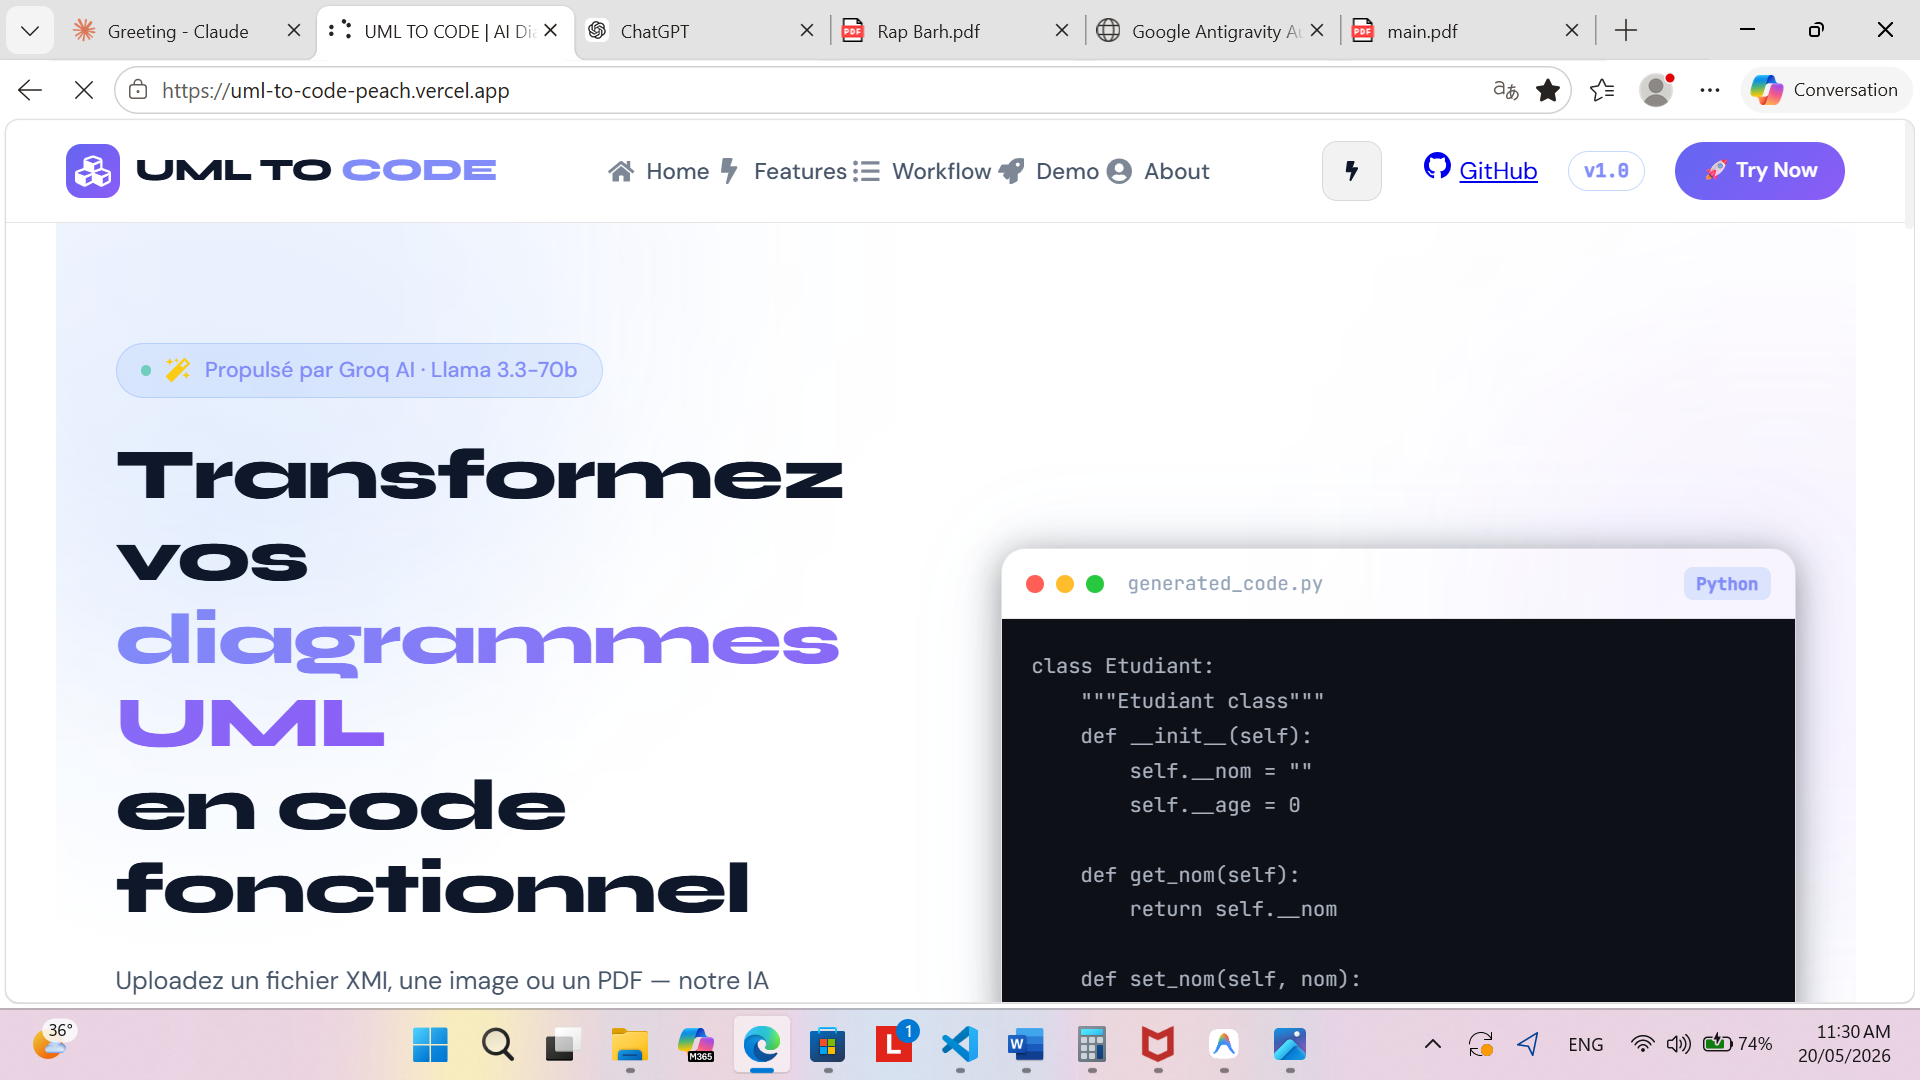
\includegraphics[width=\textwidth]{screenshots/hero.png}
    \caption{Page d'accueil — UML-to-Code (mode sombre)}
\end{figure}

\begin{figure}[H]
    \centering
    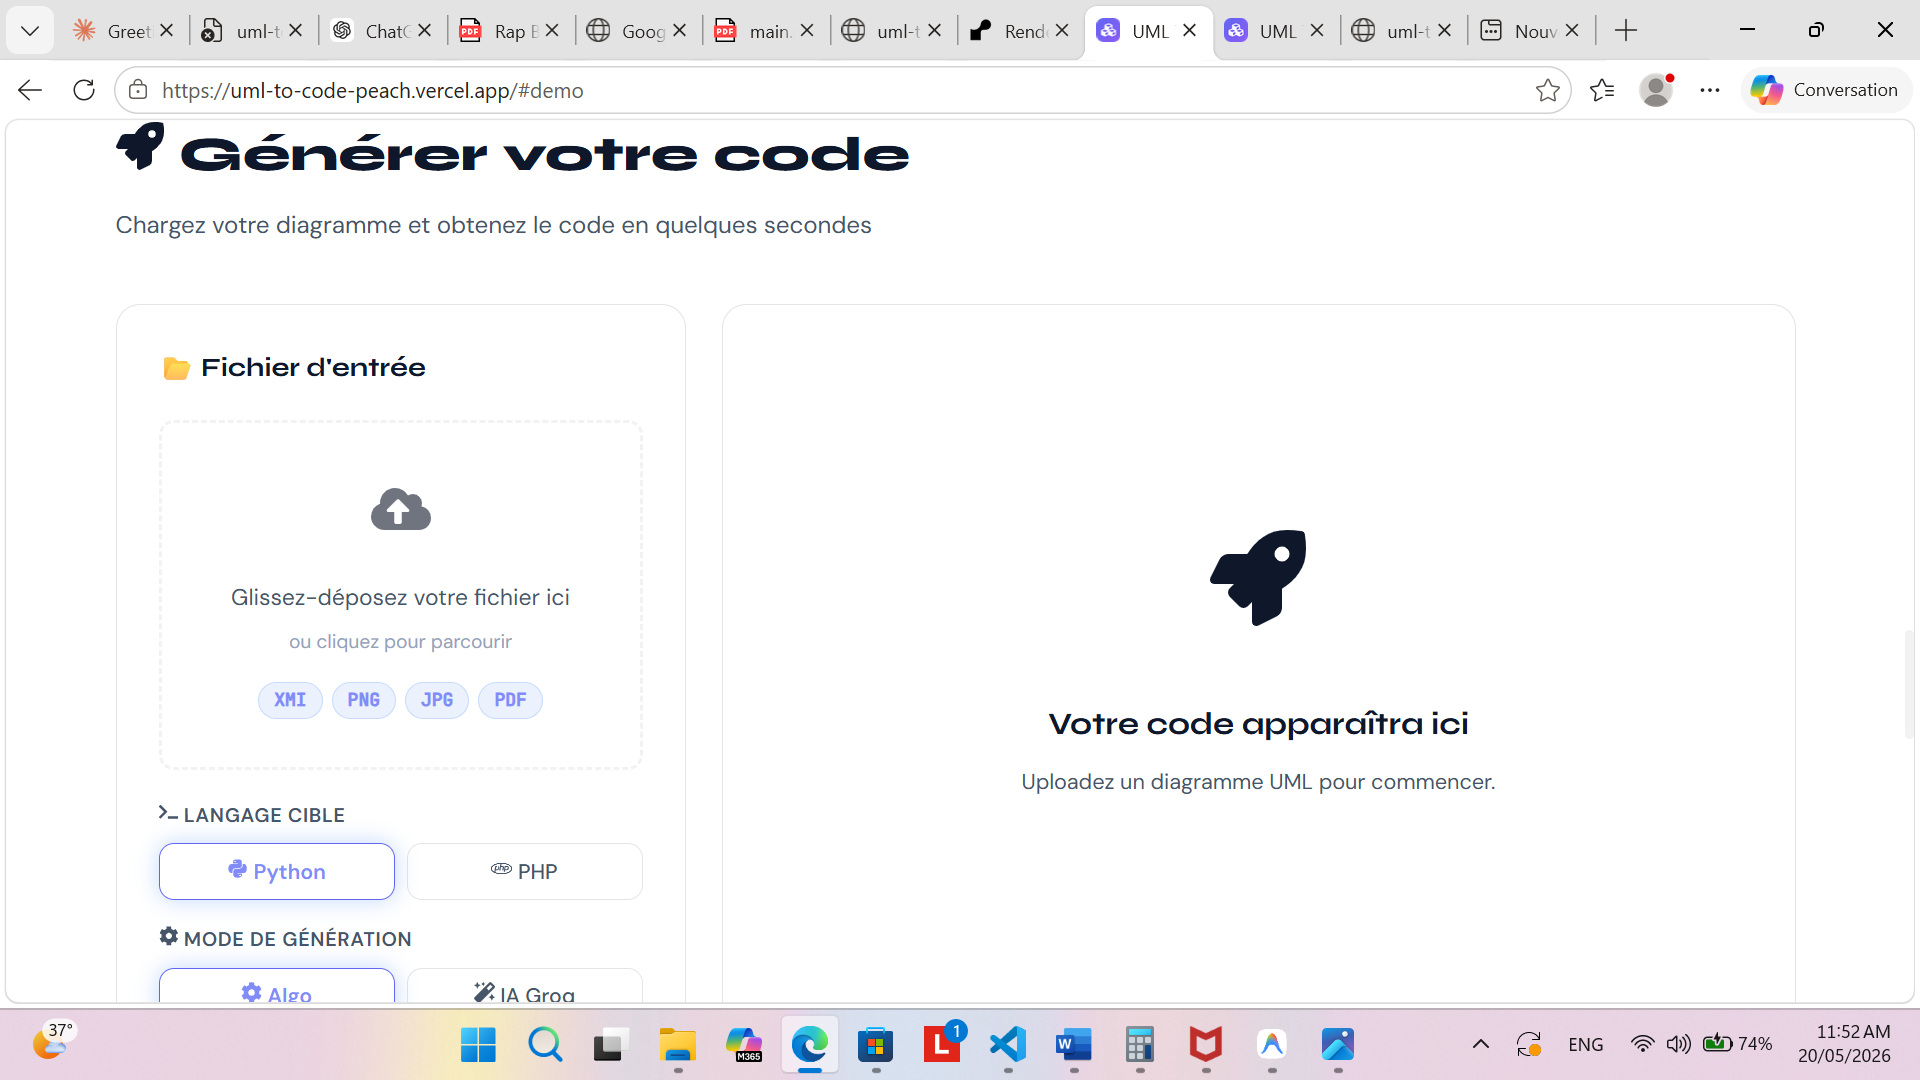
\includegraphics[width=\textwidth]{screenshots/demo.png}
    \caption{Zone de génération — Upload et Monaco Editor}
\end{figure}

\begin{figure}[H]
    \centering
    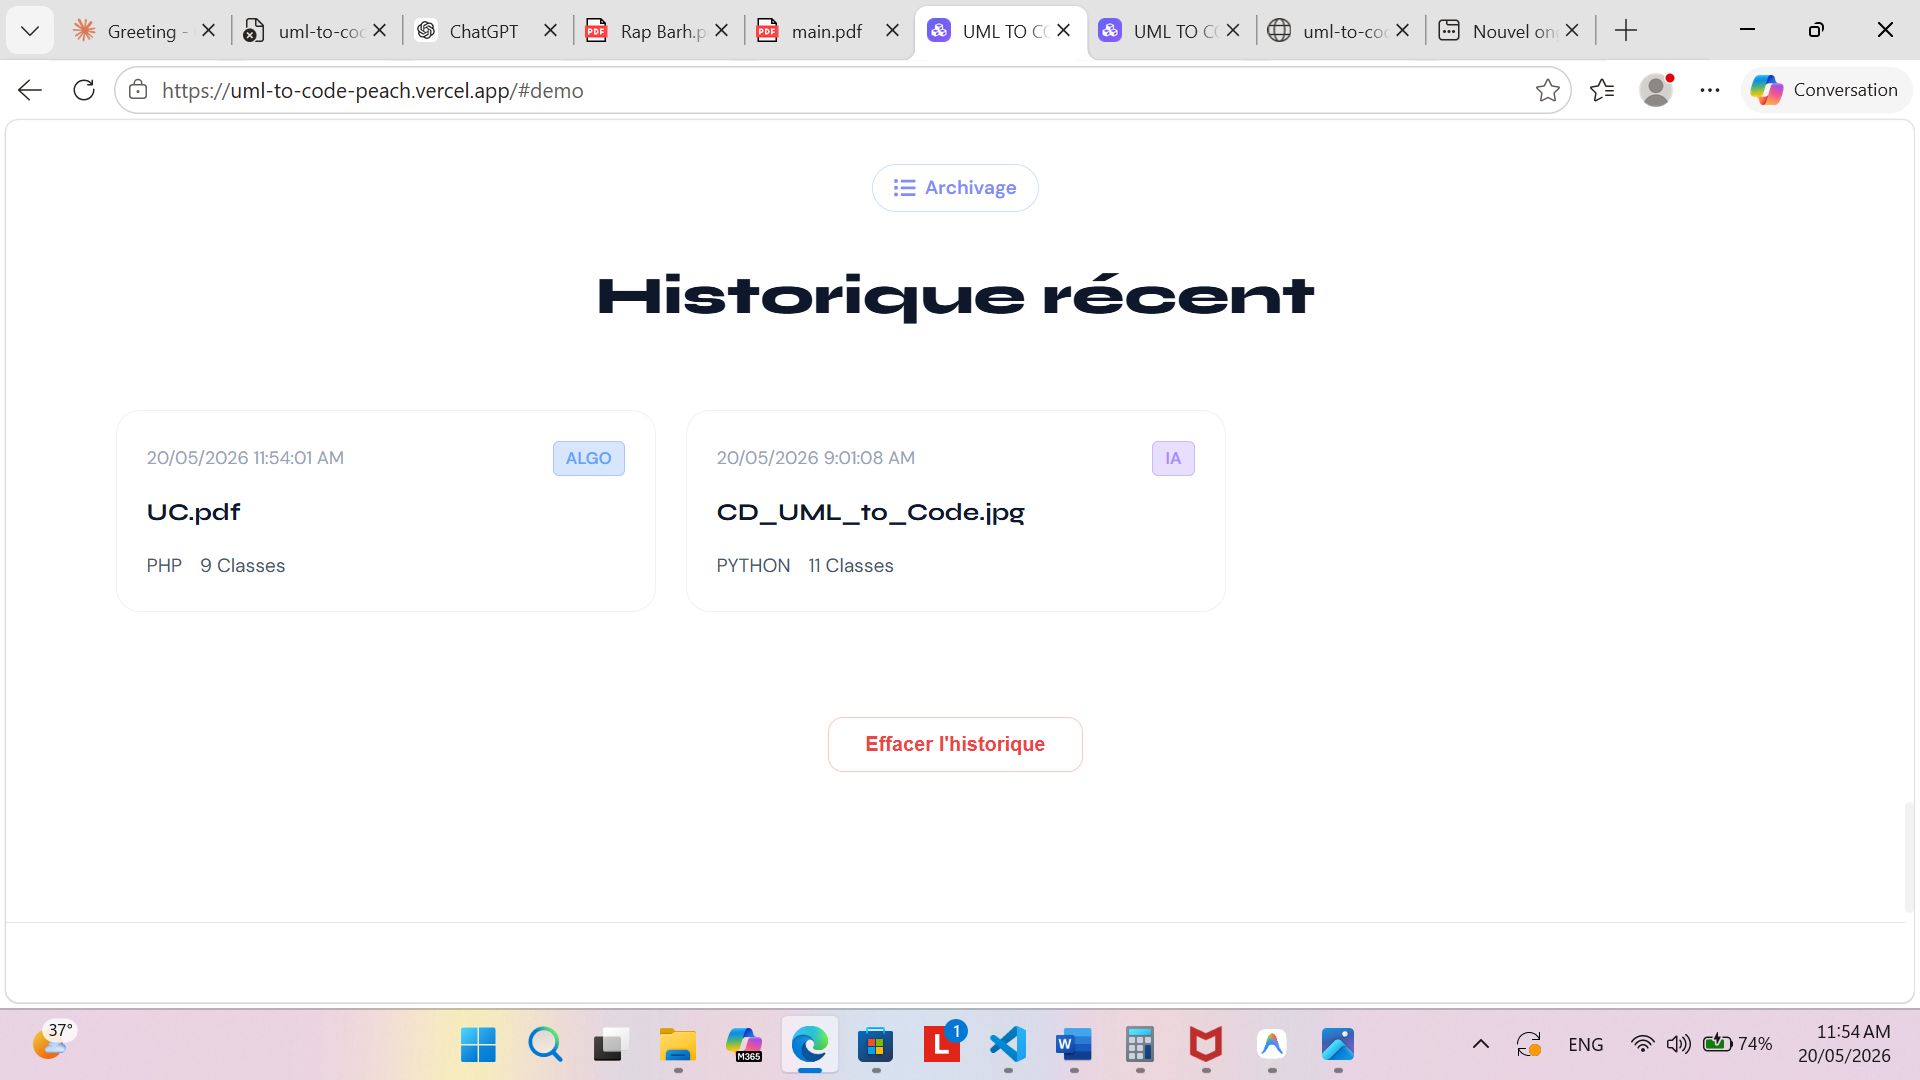
\includegraphics[width=\textwidth]{screenshots/history.png}
    \caption{Section Historique — 10 dernières générations}
\end{figure}